\chapter{Online Parameter Estimation: Adaptive Filtering}
\label{ch:adaptive_filtering}

Online parameter estimation forms the foundation of real-time monitoring, safety diagnostics, and state estimation in modern Battery Management Systems (BMS). Unlike offline characterization methods, which require long relaxation periods and controlled laboratory environments, online techniques continuously identify battery parameters under dynamic operating conditions. The parameters of an equivalent circuit model (ECM) -- specifically the ohmic resistance $R_0$, the polarization resistance $R_1$, and the polarization capacitance $C_1$ -- vary with state of charge (SOC), temperature, current rate (C-rate), and degradation state.

By tracking these parameter variations dynamically, a BMS can update its state observers in real time, leading to accurate estimates of SOC and SOH. This chapter presents the core ideas, key equations, and comparative performance of the main online parameter estimation techniques: Recursive Least Squares (RLS) and its adaptive variants, Kalman filtering formulations (EKF and UKF), and Particle Filtering. Rather than re-deriving each algorithm from first principles, the emphasis here is on the working equations an engineer actually implements and the intuition behind them; full derivations can be found in the cited references.

\begin{figure}[htbp]
\centering
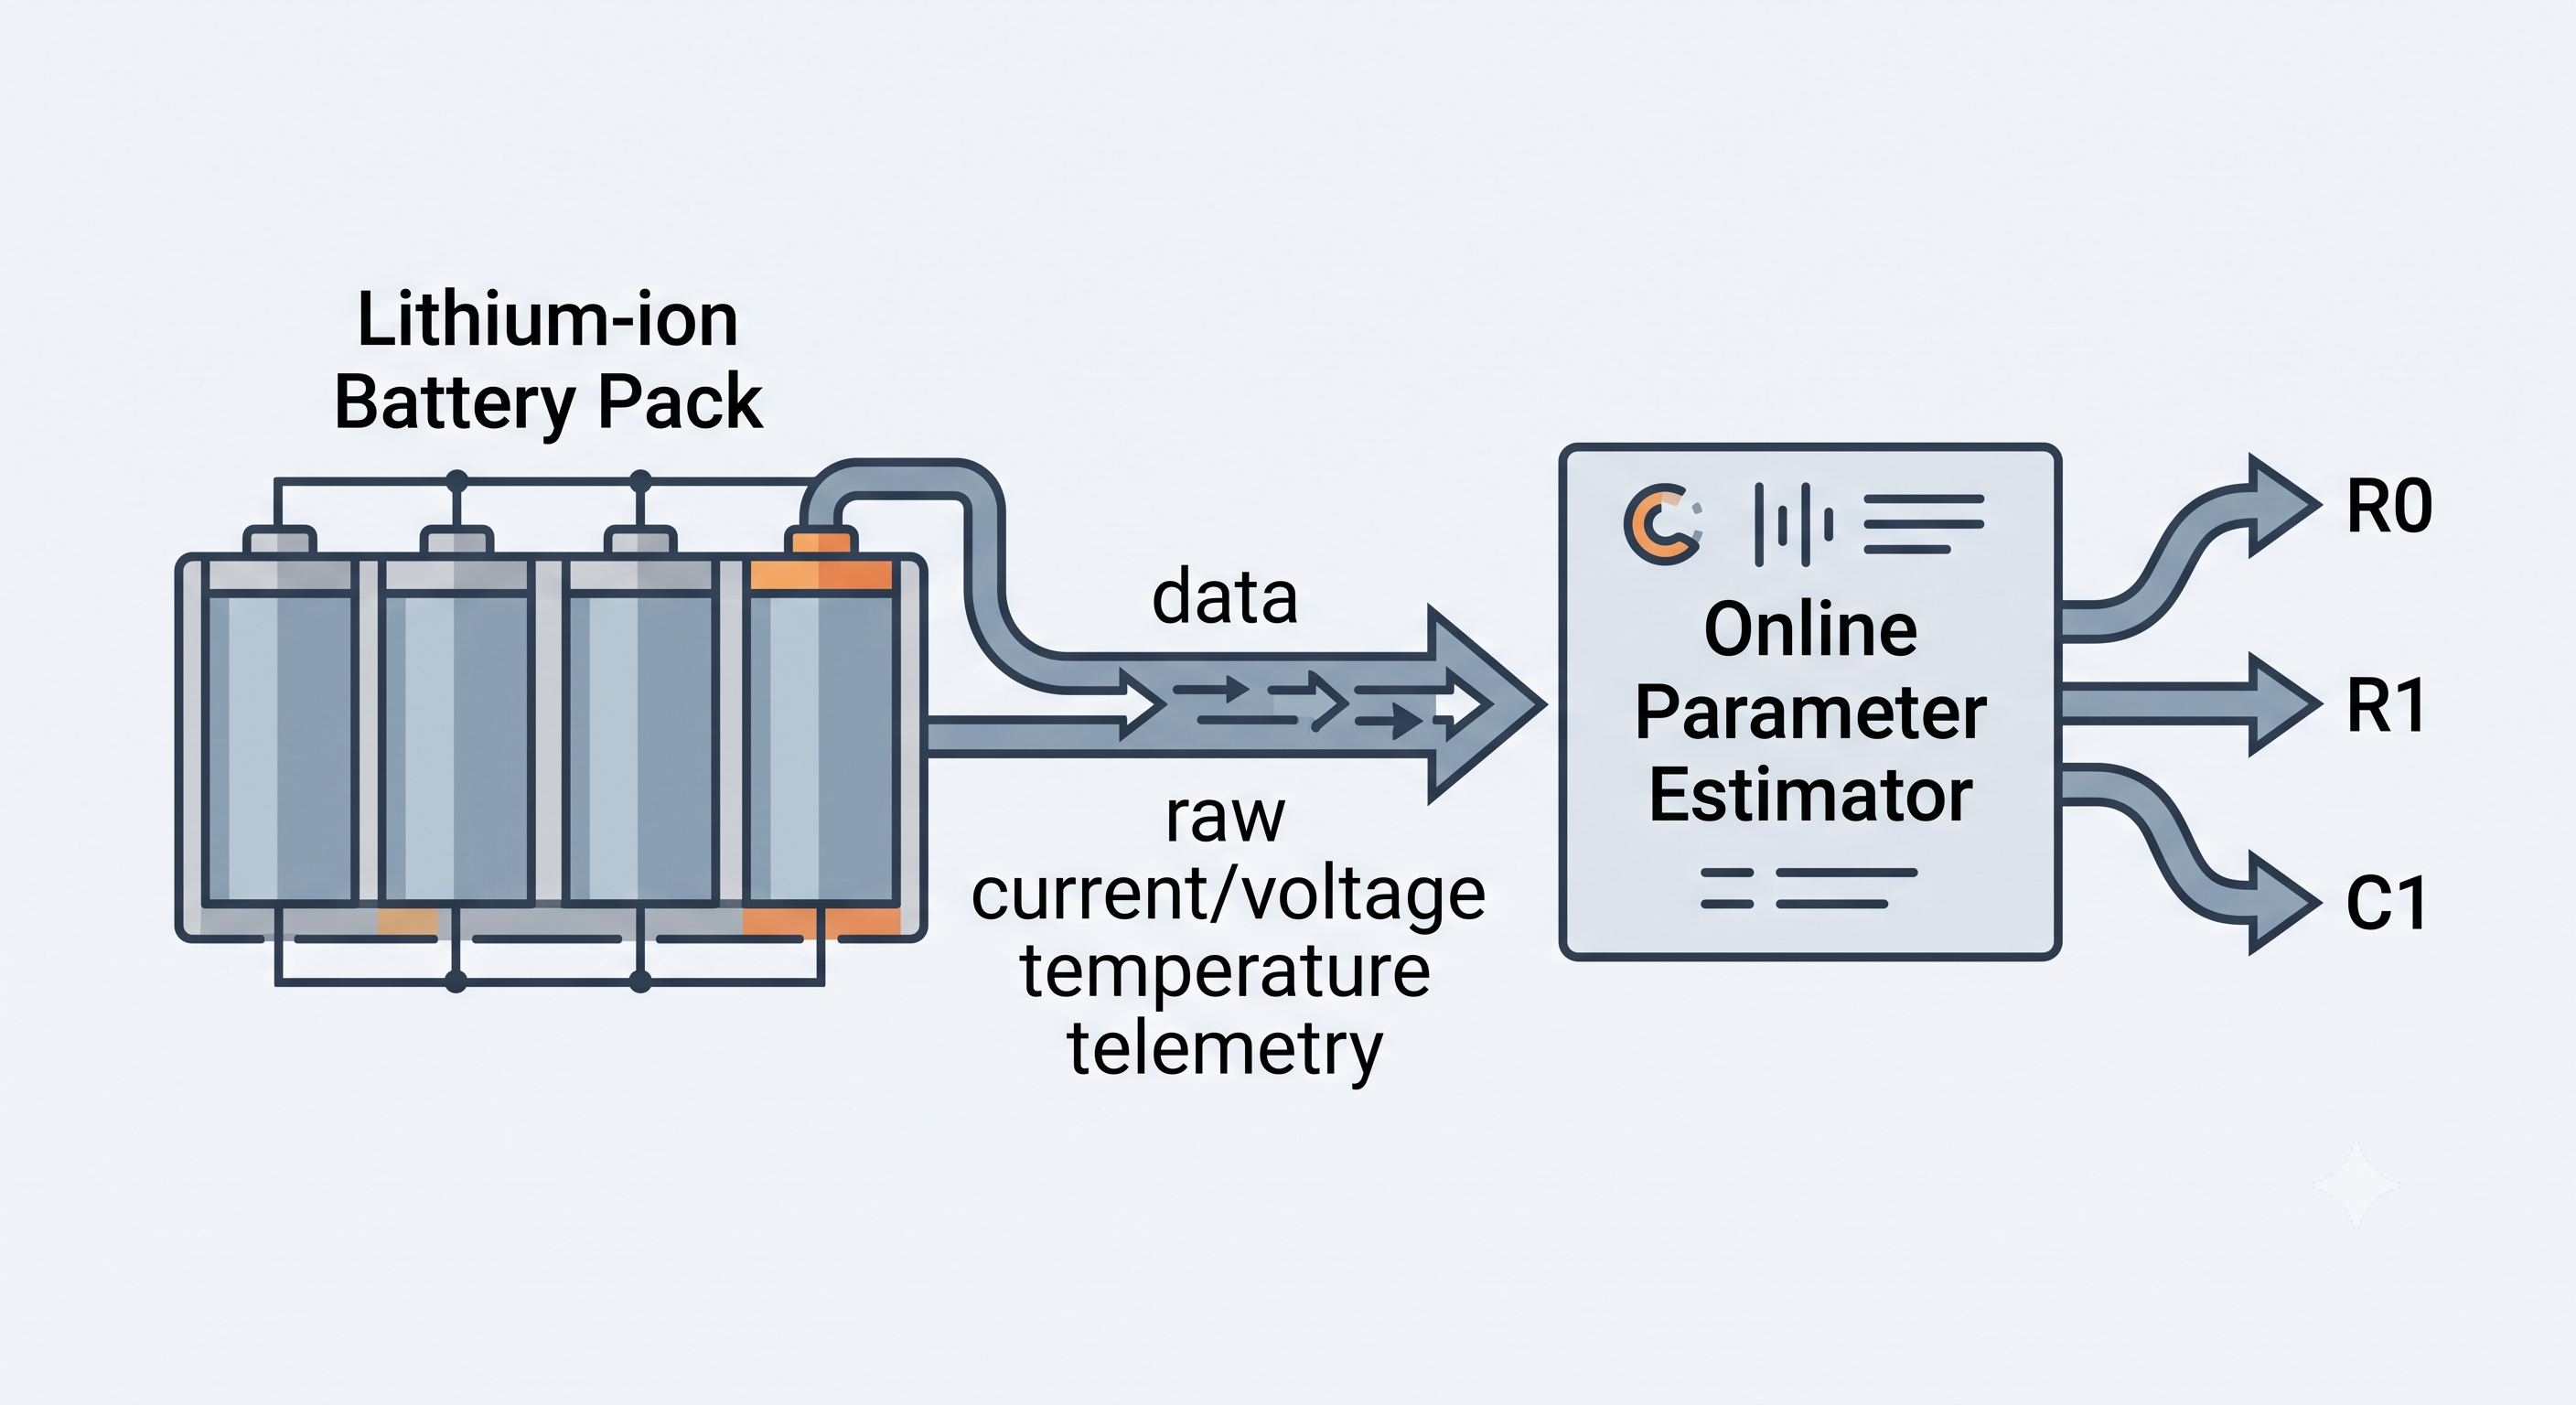
\includegraphics[width=0.65\textwidth]{ch5_img1.png}
\caption{Overview of online parameter estimation: telemetry in, ECM parameters out.}
\label{fig:ch5_overview}
\end{figure}

\section{Recursive Least Squares (RLS) and Variants}
\label{sec:rls_variants}

The Recursive Least Squares (RLS) algorithm is an online version of the offline least squares method covered in Chapter 4. Instead of solving one large regression problem after all the data has been collected, RLS updates the parameter estimate one sample at a time as new telemetry arrives. This makes it well suited to embedded systems, where the algorithm must run continuously with a small, fixed computational budget.

\subsection{ECM Discretization for RLS}
\label{subsec:ch5_discretization}

To apply RLS to a first-order Thevenin ECM, the continuous-time equations must first be written in discrete form. The continuous-time model is:
\begin{align}
V_t(t) &= V_{oc}(\text{SOC}) - V_1(t) - I(t) R_0, \label{eq:ch5_vt_cont} \\
\dot{V}_1(t) &= -\frac{1}{R_1 C_1} V_1(t) + \frac{1}{C_1} I(t). \label{eq:ch5_v1_cont}
\end{align}
Applying the bilinear (Tustin) transform to the polarization branch and rearranging terms gives the discrete-time Auto-Regressive with eXogenous input (ARX) representation:
\begin{equation}
y_k = -a_1 y_{k-1} + b_0 u_k + b_1 u_{k-1} + e_k,
\label{eq:ch5_arx}
\end{equation}
where $y_k = V_{t,k} - V_{oc}(\text{SOC}_k)$ is the OCV-compensated terminal voltage, $u_k = I_k$ is the applied current (discharge positive), and $e_k$ captures measurement noise and discretization error.

The discrete coefficients $\{a_1, b_0, b_1\}$ relate to the physical parameters $\{R_0, R_1, C_1\}$ and sampling time $T_s$ as:
\begin{align}
a_1 &= -\frac{2 R_1 C_1 - T_s}{2 R_1 C_1 + T_s}, \\
b_0 &= \frac{R_0 (2 R_1 C_1 + T_s) + R_1 T_s}{2 R_1 C_1 + T_s}, \\
b_1 &= \frac{-R_0 (2 R_1 C_1 - T_s) + R_1 T_s}{2 R_1 C_1 + T_s}.
\end{align}
Equation~\eqref{eq:ch5_arx} can be written compactly as $y_k = \boldsymbol{\phi}_k^T \boldsymbol{\theta} + e_k$, using a regressor vector $\boldsymbol{\phi}_k$ and parameter vector $\boldsymbol{\theta}$:
\begin{align}
\boldsymbol{\phi}_k &= \begin{bmatrix} -y_{k-1} & u_k & u_{k-1} \end{bmatrix}^T, \\
\boldsymbol{\theta} &= \begin{bmatrix} a_1 & b_0 & b_1 \end{bmatrix}^T.
\end{align}
Once $\hat{\boldsymbol{\theta}}_k = [\hat{a}_{1,k}, \hat{b}_{0,k}, \hat{b}_{1,k}]^T$ has been estimated, the physical ECM parameters are recovered by inverting this mapping:
\begin{align}
R_{0,k} &= \frac{\hat{b}_{0,k} - \hat{b}_{1,k}}{1 - \hat{a}_{1,k}}, \\
R_{1,k} &= \frac{2(\hat{a}_{1,k} \hat{b}_{0,k} + \hat{b}_{1,k})}{(1 - \hat{a}_{1,k})(1 + \hat{a}_{1,k})}, \\
C_{1,k} &= \frac{T_s (1 + \hat{a}_{1,k})^2}{4(\hat{a}_{1,k} \hat{b}_{0,k} + \hat{b}_{1,k})}.
\end{align}

\subsection{The Idea Behind RLS}
\label{subsec:ch5_rls_idea}

Batch least squares (Chapter 4) finds $\hat{\boldsymbol{\theta}}$ by inverting a matrix built from \emph{all} available data at once. That is fine offline, but re-inverting a growing matrix at every new time step would be far too expensive for a microcontroller. RLS avoids this by keeping a running estimate of the parameters, $\hat{\boldsymbol{\theta}}_{k-1}$, together with a small covariance matrix $\mathbf{P}_{k-1}$ that summarizes how confident the filter is in that estimate. When a new sample $(y_k, \boldsymbol{\phi}_k)$ arrives, RLS does three things: it predicts what $y_k$ \emph{should} have been using the current parameters, compares this to what was actually measured, and nudges the parameters in the direction that reduces this error -- weighted by how reliable the new information is judged to be. Using a classical result from linear algebra (the matrix inversion lemma), this update can be computed with simple matrix--vector multiplications instead of a full matrix inversion, which is what makes RLS cheap enough to run every control cycle. Ordinary RLS is simply the special case $\lambda = 1$ of the Forgetting-Factor RLS recursion presented next.

\subsection{Forgetting Factor RLS (FF-RLS)}
\label{subsec:ch5_ffrls}

For time-varying parameters, plain RLS is modified with an exponential forgetting factor $\lambda \in (0, 1]$, which weights recent measurements more heavily than old ones. The cost function minimized at time $k$ is:
\begin{equation}
J_k(\boldsymbol{\theta}) = \sum_{i=1}^k \lambda^{k-i} \left( y_i - \boldsymbol{\phi}_i^T \boldsymbol{\theta} \right)^2.
\label{eq:ffrls_cost}
\end{equation}
Minimizing this cost leads to four recursive update equations, executed once per sample:
\begin{align}
e_k &= y_k - \boldsymbol{\phi}_k^T \hat{\boldsymbol{\theta}}_{k-1}, \label{eq:ffrls_err} \\
\mathbf{K}_k &= \frac{\mathbf{P}_{k-1} \boldsymbol{\phi}_k}{\lambda + \boldsymbol{\phi}_k^T \mathbf{P}_{k-1} \boldsymbol{\phi}_k}, \label{eq:ffrls_gain} \\
\hat{\boldsymbol{\theta}}_k &= \hat{\boldsymbol{\theta}}_{k-1} + \mathbf{K}_k e_k, \label{eq:ffrls_theta} \\
\mathbf{P}_k &= \frac{1}{\lambda} \left[ \mathbf{P}_{k-1} - \mathbf{K}_k \boldsymbol{\phi}_k^T \mathbf{P}_{k-1} \right]. \label{eq:ffrls_cov}
\end{align}
Here $e_k$ is the prediction error, $\mathbf{K}_k$ is the gain vector that decides how strongly to trust the new sample, and $\mathbf{P}_k$ is the covariance matrix tracking estimator confidence.

A well-known issue with FF-RLS is \textbf{covariance wind-up}. When there is little or no excitation -- for example, the vehicle is parked and current is zero -- the regressor $\boldsymbol{\phi}_k \approx \mathbf{0}$, and Equation~\eqref{eq:ffrls_cov} reduces to $\mathbf{P}_k \approx \mathbf{P}_{k-1}/\lambda$. Since $\lambda < 1$, $\mathbf{P}_k$ grows without bound the longer the cell sits idle. When current finally does flow again, the filter treats this stale, over-confident covariance as if it were fresh, and the parameter estimate can swing wildly or diverge.

\subsection{Variable Forgetting Factor RLS (VFF-RLS)}
\label{subsec:ch5_vffrls}

To avoid wind-up, $\lambda$ can instead be adjusted dynamically based on how large the prediction error currently is:
\begin{equation}
\lambda_k = \lambda_{\min} + (1 - \lambda_{\min}) \cdot 2^{-\rho \cdot e_k^2},
\label{eq:vff_update}
\end{equation}
where $\lambda_{\min}$ is a lower bound and $\rho > 0$ is a sensitivity coefficient. A large error (indicating a real change in operating conditions) pushes $\lambda_k$ toward $\lambda_{\min}$ for fast tracking; a small, steady error lets $\lambda_k$ rise toward 1, filtering out noise once the estimate has settled.

\subsection{Directional Forgetting RLS (DF-RLS)}
\label{subsec:ch5_dfrls}

Directional forgetting takes a different approach: rather than discounting old data everywhere, it only forgets in the direction currently being excited by $\boldsymbol{\phi}_k$. The covariance update becomes:
\begin{equation}
\mathbf{P}_k = \mathbf{P}_{k-1} - \frac{\mathbf{P}_{k-1} \boldsymbol{\phi}_k \boldsymbol{\phi}_k^T \mathbf{P}_{k-1}}{\dfrac{\lambda}{1 - \lambda} + \boldsymbol{\phi}_k^T \mathbf{P}_{k-1} \boldsymbol{\phi}_k}.
\label{eq:dfrls_cov}
\end{equation}
Because directions with no new information are left untouched, $\mathbf{P}_k$ cannot grow during idle periods, which removes the wind-up problem without needing to schedule $\lambda_k$ explicitly.

\subsection{Multi-Innovation RLS (MI-RLS)}
\label{subsec:ch5_mirls}

Standard FF-RLS only looks at the single most recent sample when updating the parameters, which can make it sluggish or overly sensitive to a single noisy measurement. Multi-Innovation RLS (MI-RLS) instead looks back over a short sliding window of the last $p$ samples -- the \emph{innovation length} -- and updates the parameters using all of them together:
\begin{equation}
\mathbf{E}(p, k) = \mathbf{Y}(p, k) - \mathbf{\Phi}^T(p, k)\, \hat{\boldsymbol{\theta}}_{k-1},
\end{equation}
where $\mathbf{Y}(p,k)$ stacks the last $p$ outputs and $\mathbf{\Phi}(p,k)$ stacks the corresponding regressors. The parameter and gain updates generalize the single-sample case:
\begin{align}
\hat{\boldsymbol{\theta}}_k &= \hat{\boldsymbol{\theta}}_{k-1} + \mathbf{K}_k(p)\, \mathbf{E}(p, k), \\
\mathbf{K}_k(p) &= \mathbf{P}_{k-1} \mathbf{\Phi}(p, k) \Big[\lambda\, \mathbf{I}_{p} + \mathbf{\Phi}^T(p, k) \mathbf{P}_{k-1} \mathbf{\Phi}(p, k)\Big]^{-1}.
\end{align}
Standard RLS is simply MI-RLS with $p = 1$. Larger $p$ smooths out sensor noise and improves transient tracking, at the cost of inverting a larger $p \times p$ matrix at every step.

\subsection{Implementation of FF-RLS}
\label{subsec:ch5_ffrls_impl}

On an embedded microcontroller, the covariance matrix is typically initialized as $\mathbf{P}_0 = \gamma \mathbf{I}$, where $\gamma$ is a large scalar (e.g., $10^3$--$10^5$) representing high initial uncertainty, and $\hat{\boldsymbol{\theta}}_0$ is initialized from nominal cell values (e.g., $R_0 = 0.02~\Omega$, $R_1 = 0.015~\Omega$, $C_1 = 1000$~F). Algorithm~\ref{alg:ffrls} summarizes the per-sample execution.

\begin{algorithm}[H]
\caption{Forgetting Factor Recursive Least Squares}
\label{alg:ffrls}
\small
\begin{algorithmic}[1]
\State \textbf{Input:} telemetry $\{y_k, u_k\}$, sample time $T_s$, forgetting factor $\lambda$
\State \textbf{Output:} estimated parameters $\{R_0, R_1, C_1\}$
\State \textbf{Initialize:} $\hat{\boldsymbol{\theta}} \gets [a_{1,\mathrm{init}}, b_{0,\mathrm{init}}, b_{1,\mathrm{init}}]^T$, \quad $\mathbf{P} \gets \gamma \mathbf{I}_3$
\For{each time step $k$}
    \State $\boldsymbol{\phi}_k \gets [-y_{k-1},\, u_k,\, u_{k-1}]^T$
    \State $e_k \gets y_k - \boldsymbol{\phi}_k^T \hat{\boldsymbol{\theta}}$
    \State $\mathbf{K}_k \gets \mathbf{P} \boldsymbol{\phi}_k / \big(\lambda + \boldsymbol{\phi}_k^T \mathbf{P} \boldsymbol{\phi}_k\big)$
    \State $\hat{\boldsymbol{\theta}} \gets \hat{\boldsymbol{\theta}} + \mathbf{K}_k e_k$
    \State $\mathbf{P} \gets \big(\mathbf{P} - \mathbf{K}_k \boldsymbol{\phi}_k^T \mathbf{P}\big) / \lambda$
    \State extract $R_0, R_1, C_1$ from $\hat{\boldsymbol{\theta}}$ using the mapping in \S\ref{subsec:ch5_discretization}
    \State $y_{k-1} \gets y_k$, \quad $u_{k-1} \gets u_k$
\EndFor
\end{algorithmic}
\end{algorithm}

\begin{figure}[H]
\centering
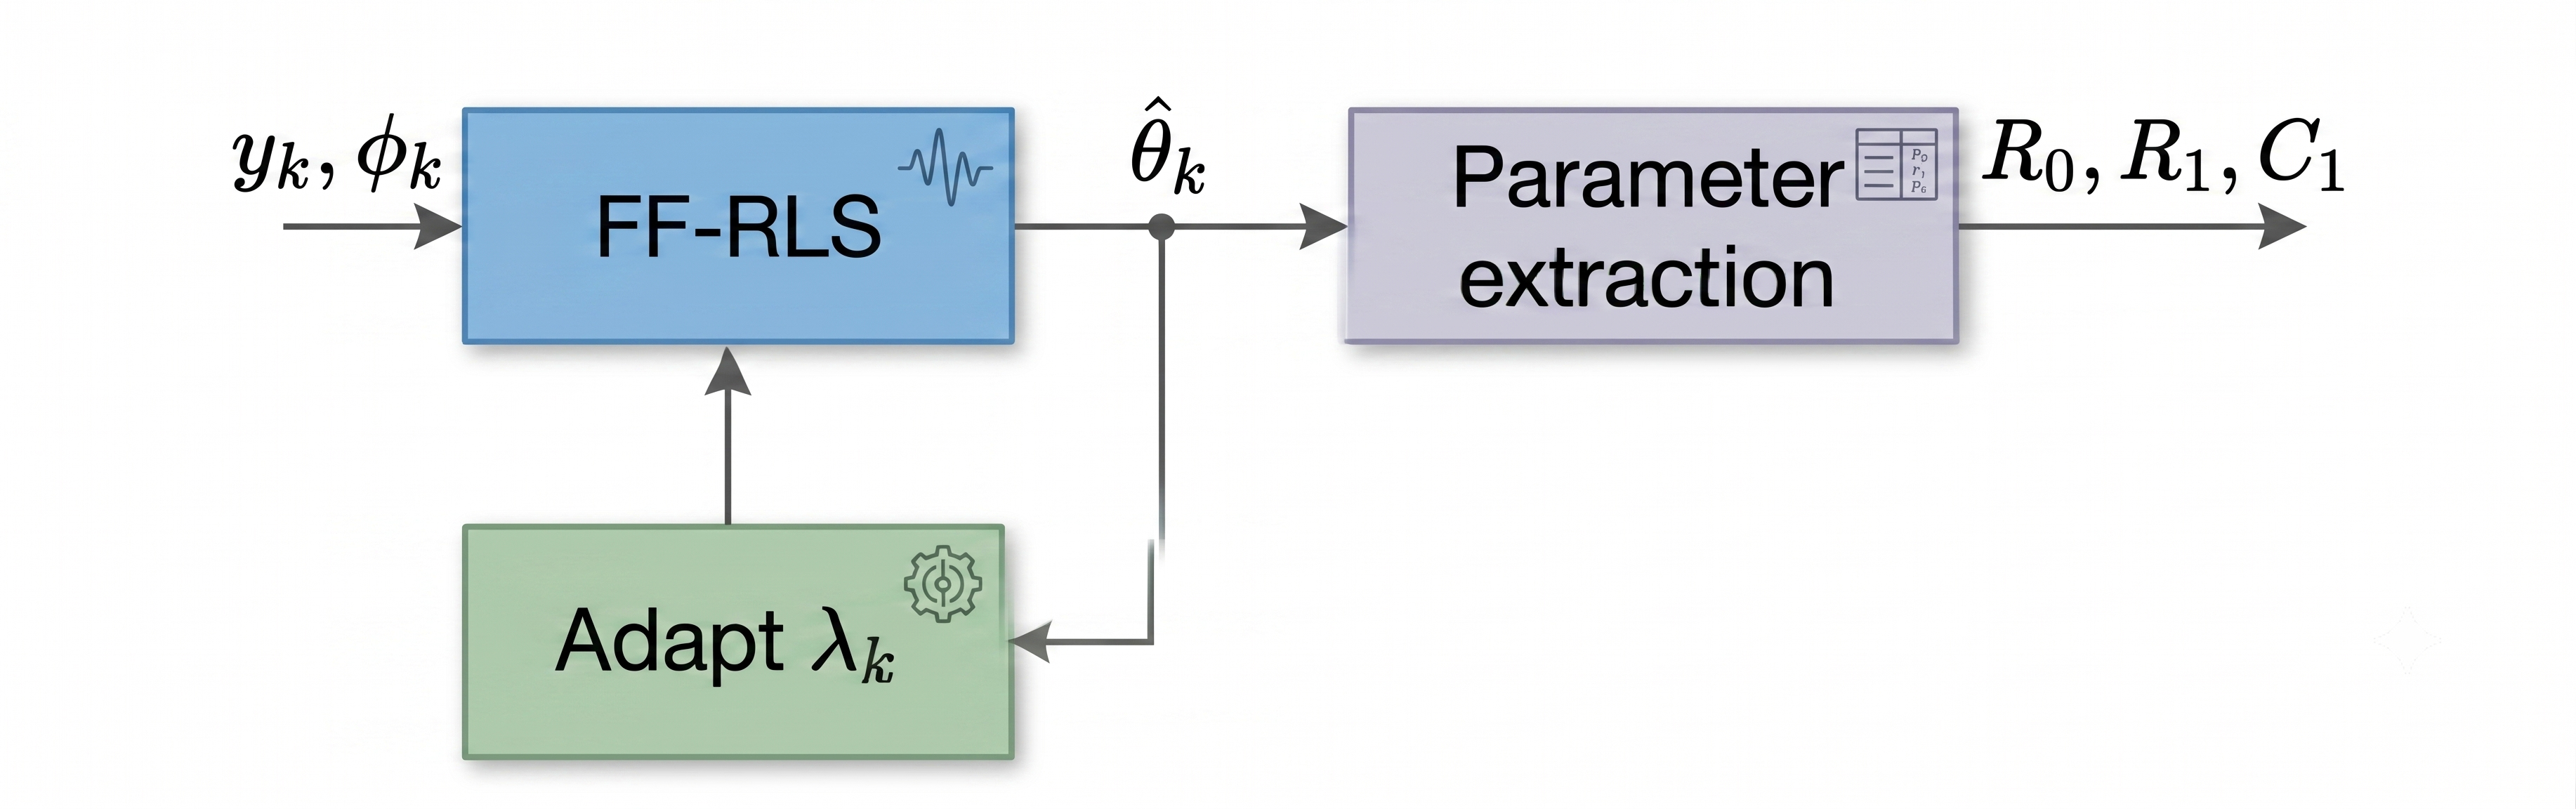
\includegraphics[width=0.7\textwidth]{figure5.2.png}


\caption{Block diagram of the adaptive RLS parameter estimation loop.}
\label{fig:rls_block}
\end{figure}

\section{Kalman Filter Formulations}
\label{sec:kalman_formulations}

Kalman filtering takes a state-space approach to estimation. By explicitly modeling system dynamics and sensor noise, it computes the state estimate that minimizes mean-square error. For battery applications, parameters are treated either as extra states appended to the state vector (Joint Kalman Filtering) or estimated by a separate filter running in parallel (Dual Kalman Filtering). The underlying discrete-time non-linear model is:
\begin{align}
\mathbf{x}_k &= f(\mathbf{x}_{k-1}, u_{k-1}) + \mathbf{w}_{k-1}, \\
y_k &= g(\mathbf{x}_k, u_k) + v_k,
\end{align}
where $\mathbf{x}_k$ is the state vector, $u_k$ the input current, $y_k$ the terminal voltage, and $\mathbf{w}_k, v_k$ are process and measurement noise with covariances $\mathbf{Q}_k$ and $R_k$.

\subsection{Extended Kalman Filter (EKF)}
\label{subsec:ekf_details}

The EKF linearizes $f$ and $g$ at each time step using their Jacobians, $\mathbf{F}_{k-1} = \partial f/\partial \mathbf{x}$ and $\mathbf{H}_k = \partial g/\partial \mathbf{x}$, evaluated at the current estimate. For joint estimation, the augmented state is $\mathbf{x}_{a,k} = [\text{SOC}_k, V_{1,k}, R_{0,k}, R_{1,k}, C_{1,k}]^T$. Each time step runs a predict--update cycle, one equation at a time:
\begin{align}
\hat{\mathbf{x}}_{k|k-1} &= f(\hat{\mathbf{x}}_{k-1|k-1}, u_{k-1}), \label{eq:ekf_predict_x}\\
\mathbf{P}_{k|k-1} &= \mathbf{F}_{k-1} \mathbf{P}_{k-1|k-1} \mathbf{F}_{k-1}^T + \mathbf{Q}_{k-1}, \label{eq:ekf_predict_p}\\
\mathbf{K}_k &= \mathbf{P}_{k|k-1} \mathbf{H}_k^T \big(\mathbf{H}_k \mathbf{P}_{k|k-1} \mathbf{H}_k^T + R_k\big)^{-1}, \label{eq:ekf_gain}\\
\hat{\mathbf{x}}_{k|k} &= \hat{\mathbf{x}}_{k|k-1} + \mathbf{K}_k\big(y_k - g(\hat{\mathbf{x}}_{k|k-1}, u_k)\big), \label{eq:ekf_update_x}\\
\mathbf{P}_{k|k} &= (\mathbf{I} - \mathbf{K}_k \mathbf{H}_k)\, \mathbf{P}_{k|k-1}. \label{eq:ekf_update_p}
\end{align}
The first two lines are the \emph{predict} step, and the last three are the \emph{update} step once a new voltage measurement $y_k$ arrives. Because linearization is only a local approximation, the EKF can lose accuracy -- or even diverge -- when the true dynamics are strongly non-linear, such as along the flat OCV curve of $\text{LiFePO}_4$ cells.

\subsection{Unscented Kalman Filter (UKF)}
\label{subsec:ukf_details}

The UKF avoids linearization altogether. Instead of computing Jacobians, it selects a small set of representative points around the current estimate -- \textbf{sigma points} -- and passes each one through the true, non-linear functions $f$ and $g$. The mean and covariance of the resulting outputs are then reconstructed from these propagated points, which captures the effect of the non-linearity far more accurately than a first-order linear approximation, at a similar computational cost to the EKF.

For an $L$-dimensional state with mean $\hat{\mathbf{x}}_k$ and covariance $\mathbf{P}_k$, $2L+1$ sigma points are generated symmetrically around $\hat{\mathbf{x}}_k$ using the matrix square root of $\mathbf{P}_k$, scaled by a tuning parameter $\lambda_{ut}$. Each sigma point is propagated through $f$ to predict the next state, and through $g$ to predict the corresponding measurement; the predicted mean and covariance in each case are simply the weighted average of the propagated points. From these, a cross-covariance $\mathbf{P}_{xy,k}$ between the state and the predicted measurement is computed, and the filter update follows the same structure as the EKF, applied one line at a time:
\begin{align}
\mathbf{K}_k &= \mathbf{P}_{xy,k}\, \mathbf{P}_{yy,k}^{-1}, \\
\hat{\mathbf{x}}_{k|k} &= \hat{\mathbf{x}}_{k|k-1} + \mathbf{K}_k\big(y_k - \hat{y}_{k|k-1}\big), \\
\mathbf{P}_{k|k} &= \mathbf{P}_{k|k-1} - \mathbf{K}_k \mathbf{P}_{yy,k} \mathbf{K}_k^T.
\end{align}

\begin{figure}[htbp]
\centering
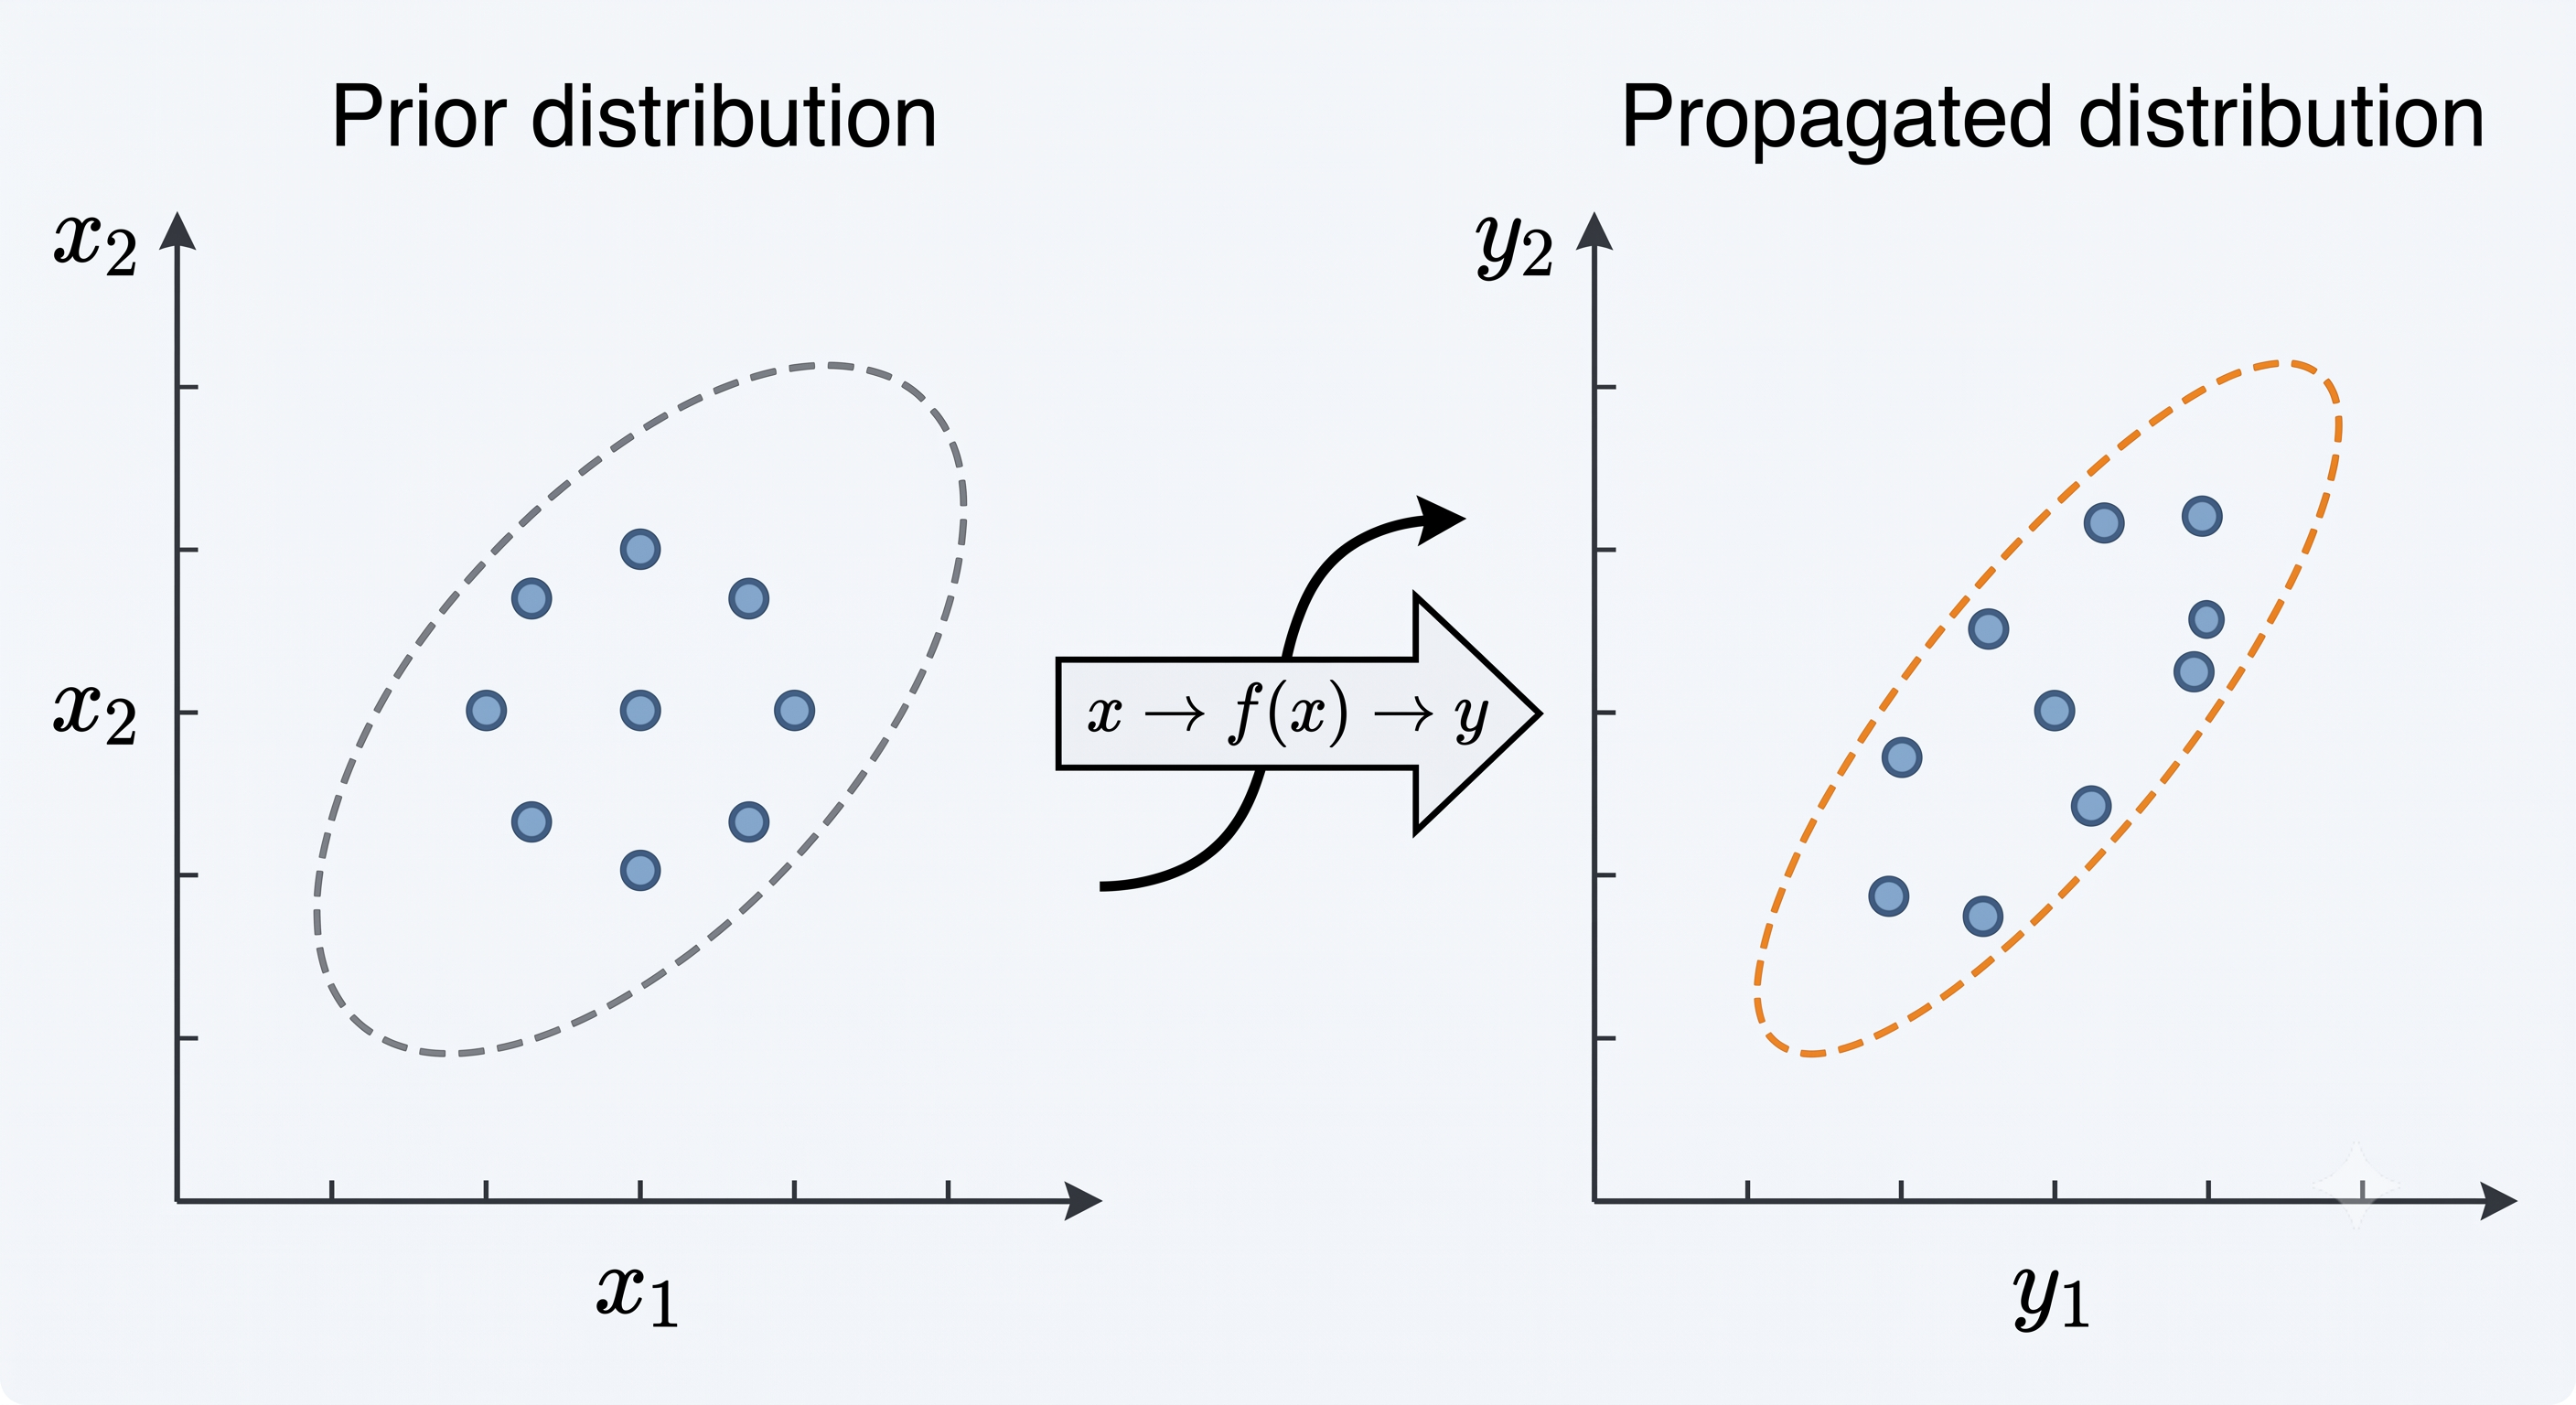
\includegraphics[width=0.7\textwidth]{ch5_img2.png}
\caption{Sigma points before and after propagation through a non-linear function in the UKF.}
\label{fig:ukf_sigma}
\end{figure}

\subsection{Tuning the UKF}
\label{subsec:ch5_ukf_tuning}

Filter performance depends heavily on the choice of $\mathbf{Q}$ and $R$:
\begin{itemize}
    \item \textbf{Process noise $\mathbf{Q}$:} larger values let the filter follow rapid parameter changes but produce noisier estimates. Slowly varying parameters (e.g., $R_1, C_1$) are usually given smaller process noise than the faster-moving $R_0$.
    \item \textbf{Measurement noise $R$:} a larger value tells the filter to trust its own model prediction over the sensor reading, which slows convergence but rejects more measurement noise.
\end{itemize}

Algorithm~\ref{alg:joint_ukf} summarizes the joint UKF execution used for combined state and parameter tracking.

\begin{algorithm}[htbp]
\caption{Joint Unscented Kalman Filter}
\label{alg:joint_ukf}
\small
\begin{algorithmic}[1]
\State \textbf{Input:} telemetry $\{y_k, u_k\}$, process covariance $\mathbf{Q}$, measurement covariance $R$
\State \textbf{Output:} joint state estimate $\hat{\mathbf{x}}_k$
\State \textbf{Initialize:} $\hat{\mathbf{x}}_0 \gets [\text{SOC}_0, V_{1,0}, R_{0,0}, R_{1,0}, C_{1,0}]^T$, \quad $\mathbf{P}_0 \gets \mathbf{P}_{\text{initial}}$
\For{each time step $k$}
    \State generate sigma points from $\hat{\mathbf{x}}_{k-1}$ and $\mathbf{P}_{k-1}$
    \State propagate sigma points through $f(\cdot, u_{k-1})$; compute $\hat{\mathbf{x}}_{k|k-1}$, $\mathbf{P}_{k|k-1}$
    \State propagate the same sigma points through $g(\cdot, u_k)$; compute $\hat{y}_k$, $\mathbf{P}_{yy}$, $\mathbf{P}_{xy}$
    \State $\mathbf{K}_k \gets \mathbf{P}_{xy} \mathbf{P}_{yy}^{-1}$
    \State $\hat{\mathbf{x}}_k \gets \hat{\mathbf{x}}_{k|k-1} + \mathbf{K}_k (y_k - \hat{y}_k)$
    \State $\mathbf{P}_k \gets \mathbf{P}_{k|k-1} - \mathbf{K}_k \mathbf{P}_{yy} \mathbf{K}_k^T$
\EndFor
\end{algorithmic}
\end{algorithm}

\section{Particle Filtering}
\label{sec:particle_filtering}

For systems with strongly non-linear dynamics or non-Gaussian noise, Particle Filtering (Sequential Monte Carlo) offers a more general alternative to Kalman-family filters. It represents the posterior distribution $p(\mathbf{x}_k \mid y_{1:k})$ using a set of $N_p$ weighted random samples, or \emph{particles}:
\begin{equation}
p(\mathbf{x}_k \mid y_{1:k}) \approx \sum_{j=1}^{N_p} w_k^{(j)}\, \delta\big(\mathbf{x}_k - \mathbf{x}_k^{(j)}\big),
\end{equation}
where $\mathbf{x}_k^{(j)}$ is the state of particle $j$ and $w_k^{(j)}$ its normalized weight. Weights are updated using the measurement likelihood,
\begin{equation}
w_k^{(j)} \propto w_{k-1}^{(j)} \cdot p\big(y_k \mid \mathbf{x}_k^{(j)}\big),
\end{equation}
which, for Gaussian measurement noise, takes the familiar bell-curve form
\begin{equation}
p\big(y_k \mid \mathbf{x}_k^{(j)}\big) = \frac{1}{\sqrt{2\pi R_k}} \exp\!\left( -\frac{\big(y_k - g(\mathbf{x}_k^{(j)}, u_k)\big)^2}{2 R_k} \right).
\end{equation}

A well-known problem is \textbf{weight degeneracy}: after enough steps, nearly all the weight concentrates on a handful of particles while the rest become useless. This is monitored using the effective sample size,
\begin{equation}
N_{\text{eff}} = \frac{1}{\sum_{j=1}^{N_p} \big(w_k^{(j)}\big)^2}.
\end{equation}
When $N_{\text{eff}}$ falls below a threshold (typically $N_p/2$), \textbf{resampling} is triggered: low-weight particles are discarded and replaced with copies of high-weight ones, refocusing computational effort where it matters.

\subsection{Systematic Resampling}
\label{subsec:ch5_resampling}

Systematic resampling is the most common choice for embedded use because it is simple and has low computational overhead. It divides the interval $[0,1)$ into $N_p$ equal segments and draws only a single random number, rather than one per particle:

\begin{enumerate}
    \item Compute the cumulative sum of the particle weights, $c = \mathrm{cumsum}(w_k)$.
    \item Draw one random starting point $u_1 \sim \mathcal{U}(0,\, 1/N_p)$.
    \item For each output particle $j = 1, \dots, N_p$: compute $u_j = u_1 + (j-1)/N_p$, advance an index pointer through $c$ until $c(i) \geq u_j$, and copy particle $i$ into the new set with weight $1/N_p$.
\end{enumerate}

Table~\ref{tab:resampling_comparison} compares this scheme against the other common resampling strategies.

\begin{table}[htbp]
\centering
\caption{Comparison of resampling methods for particle filters.}
\label{tab:resampling_comparison}
\footnotesize
\begin{tabularx}{\textwidth}{
    >{\raggedright\arraybackslash}p{2.4cm}
    >{\raggedright\arraybackslash}p{2.2cm}
    >{\raggedright\arraybackslash}X
}
\toprule
\textbf{Method} & \textbf{Complexity} & \textbf{Suitability for BMS hardware} \\
\midrule
Multinomial & $\mathcal{O}(N_p \log N_p)$, high variance & Poor -- sorting/search overhead \\
Systematic & $\mathcal{O}(N_p)$, low variance & Excellent -- simple loop structure \\
Stratified & $\mathcal{O}(N_p)$, low variance & Good -- slightly more random draws \\
Residual & $\mathcal{O}(N_p)$, very low variance & Moderate -- needs two allocation stages \\
\bottomrule
\end{tabularx}
\end{table}

\section{Summary}
\label{sec:ch5_summary}

Online parameter estimation is essential for keeping a battery model accurate as operating conditions change. The available algorithms span a wide range, from the lightweight RLS family to the more robust but computationally heavier particle filter. Table~\ref{tab:ch5_summary} summarizes their key characteristics.

\begin{table}[htbp]
\centering
\caption{Characteristics of online parameter estimation algorithms.}
\label{tab:ch5_summary}
\footnotesize
\begin{tabularx}{\textwidth}{
    >{\raggedright\arraybackslash}p{2.6cm}
    >{\raggedright\arraybackslash}p{1.6cm}
    >{\raggedright\arraybackslash}X
}
\toprule
\textbf{Algorithm} & \textbf{Cost} & \textbf{Key advantage / disadvantage} \\
\midrule
RLS / FF-RLS & Low & Fast convergence; susceptible to covariance wind-up \\
VFF-RLS / DF-RLS & Low--medium & Prevents wind-up dynamically \\
EKF & Medium & Simple state-space structure; linearization errors near flat OCV \\
UKF & Medium--high & More accurate than EKF; avoids Jacobian calculations \\
Particle Filter & High & Handles arbitrary non-linearities and non-Gaussian noise; heaviest computational load \\
\bottomrule
\end{tabularx}
\end{table}

\subsection{Algorithm Selection for BMS}
\label{subsec:ch5_selection}

The right choice depends on the balance between processing constraints and estimation requirements. For \textbf{low-cost microcontrollers}, Variable Forgetting Factor RLS is usually the most practical option, needing minimal RAM and execution time. For \textbf{high-performance BMS platforms}, Dual or Joint UKF gives the best balance of accuracy and tracking speed under demanding, dynamic conditions.

These families are not competing alternatives so much as complementary tools occupying different points on the accuracy-versus-complexity trade-off. Production hardware tends to prioritize numerical robustness and predictable execution time, while research or high-performance platforms can afford to trade extra computation for faster convergence, lower linearization error, and better handling of non-Gaussian uncertainty. This chapter establishes the core engineering intuition that underpins the observer-based and co-estimation frameworks developed in the chapters that follow.

Observers, presented in Chapter~6, offer an alternative, control-theoretic perspective on the same estimation problem.